\documentclass[8pt,a4paper]{extarticle}

\setcounter{tocdepth}{2}


\usepackage[utf8]{inputenc}
\usepackage[T1]{fontenc}
\usepackage[english]{babel}
\usepackage{geometry}
\geometry{margin=2.0cm}
\usepackage{array}
\usepackage{float}
\usepackage{placeins}
\usepackage{pdflscape}
\usepackage{csvsimple}
\usepackage{longtable}
\usepackage{pgfmath}
\usepackage{csquotes}

\usepackage{amsmath}

\newcommand{\hardswish}{\operatorname{h-swish}}
\newcommand{\relu}{\operatorname{ReLU}}
\newcommand{\sigmoid}{\operatorname{\sigma}}
\newcommand{\tablevalue}[1]{\pgfmathprintnumber[fixed,precision=3]{#1}}

\usepackage[backend=bibtex, style=ieee]{biblatex}
\addbibresource{./bibliography.bib}

\usepackage{caption}
\usepackage{subcaption}

\usepackage{booktabs}
\usepackage{graphicx}
\usepackage{amssymb}
\usepackage{multirow}
\usepackage{amsopn}

\title{
    \textbf{Project I - Logistic regression} \\[0.5cm]
    \large Advanced Machine Learning
}
\author{Igor Rudolf \and Michał Szewczak \and Sebastian Trojan}
\date{\today}

\begin{document}

\maketitle
\newpage
\begin{abstract}
This report studies binary classification with partially missing training labels, focusing on logistic-regression-based approaches under different missingness mechanisms. We compare four methods: an Oracle model trained on complete labels, a Naive model trained only on observed labels, and two variants of \texttt{UnlabeledLogReg} that first complete missing labels using either logistic regression or $k$-nearest neighbours and then fit a FISTA-based logistic lasso classifier. Experiments are conducted on four benchmark datasets under four standard missingness settings: \texttt{MCAR}, \texttt{MAR1}, \texttt{MAR2}, and \texttt{MNAR}. Performance is evaluated using accuracy, balanced accuracy, F1 score, and ROC AUC across five random seeds.

The results show that the effect of missing labels is strongly dataset-dependent and that no single practical method dominates in all settings. On easier datasets such as \texttt{breast\_cancer} and \texttt{spambase}, the Naive baseline remains highly competitive, especially under \texttt{MCAR}, \texttt{MAR1}, and \texttt{MAR2}. In contrast, logistic label completion becomes more beneficial in difficult settings, particularly under \texttt{MNAR}, where missingness depends on the label itself. The most distinctive behavior appears on \texttt{madelon}, where the unlabeled methods substantially outperform both baseline approaches. Overall, the study shows that both the missingness mechanism and the dataset structure play a crucial role in determining whether label completion is helpful.
\end{abstract}
\newpage
\tableofcontents
\newpage
\section{Project Goal}
This project studies binary classification when part of the training labels are missing. In this setting, feature vectors are available for all observations, but class labels are observed only for a subset of the training data. As a result, standard supervised methods cannot be applied directly without either discarding unlabeled examples or introducing an additional mechanism for handling the missing labels.

The main goal of the project is to evaluate whether recovering missing labels can improve downstream classification performance. To this end, we focus on logistic-regression-based methods and compare several approaches: an Oracle model trained on complete labels, a Naive model trained only on the observed subset, and unlabeled-learning variants that first complete missing labels and then fit the final classifier. The comparison is carried out under controlled missingness mechanisms, allowing us to assess not only which method performs best on average, but also under which datasets and missingness settings label completion is most beneficial.
\section{Data Description}
We conducted our experiments on the following datasets:
\begin{itemize}
    \item \textbf{Wisconsin Breast Cancer} -  dataset consists of 30 features computed from a digitized image of a fine needle aspirate (FNA) of a breast mass. The features describe characteristics of the cell nuclei present in the image, such as radius, texture, perimeter, and area, and are used to classify them as Malignant or Benign. The dataset has 569 instances. 
    \item \textbf{Ionosphere} - Collected by a phased array of 16 high-frequency antennas in Goose Bay, Labrador, this dataset targets free electrons in the ionosphere, with 34 attributes in each record. "Good" radar returns show evidence of some type of structure in the ionosphere, while "Bad" returns do not. The dataset has 569 instances. 
    \item \textbf{Spambase} - This dataset contains 57 features derived from emails to determine if they are "Spam" or "Non-Spam." Attributes include the frequency of specific words and characters, as well as statistics regarding sequences of capital letters. The dataset has 4601 instances. 
    \item \textbf{Madelon}  Madelon is an artificial dataset created for the NIPS 2003 Feature Selection Challenge. It is a highly non-linear dataset with most (480 of 500) features being noise features. The dataset has 4400 instances.
\end{itemize}
\section{Missingness Generators}

We implemented four missing-label generators corresponding to the standard settings \texttt{MCAR}, \texttt{MAR1}, \texttt{MAR2}, and \texttt{MNAR}. In all cases, the generator returns a partially observed training label vector in which missing labels are encoded as $-1$.

The \texttt{MCAR} generator (\emph{Missing Completely At Random}) removes labels independently of both the input features and the true class. For each training example, the label is replaced by a missing value with probability equal to the selected \texttt{missing\_rate}. This is the simplest setting and serves as a baseline for random label loss.

The \texttt{MAR1} generator (\emph{Missing At Random}) makes the probability of a missing label depend on a single selected feature. More precisely, the missingness probability is defined by a logistic function of one feature column, and the bias term is chosen so that the average missing-label fraction is close to the required target rate. In this way, the chance that a label is missing depends on the observed covariates but not directly on the true label.

The \texttt{MAR2} generator extends this idea by using a weighted linear combination of all features instead of only one feature. As in \texttt{MAR1}, the missingness probability is given by a logistic function, with its bias adjusted to match the desired average missing rate. This produces a more complex feature-dependent missingness pattern.

Finally, the \texttt{MNAR} generator (\emph{Missing Not At Random}) makes missingness depend directly on label-related information. In our implementation, a logistic-regression model is first fitted to estimate class probabilities, and these probabilities are then combined with the true binary labels to construct per-sample missingness probabilities. The resulting probabilities are rescaled to achieve the requested average missing rate. This setting is the most difficult, because missingness is no longer explained only by the observed features.

\section{FISTA Logistic Regression Implementation}
\subsection{Optimizer}
The core of our logistic regression implementation is the optimizer which uses Fast Iterative Shrinkage-Thresholding Algorithm (FISTA) to learn the weights of the model by optmizing the function \begin{equation}
     -\frac{1}{n} \sum_{i=1}^{n} \left[ y_i \ln(\sigma(\mathbf{x}_i^T \mathbf{w})) + (1 - y_i) \ln(1 - \sigma(\mathbf{x}_i^T \mathbf{w})) \right] + \lambda \sum_{j=1}^{p} |w_j|
\end{equation}. This can be expressed as the sum of a smooth convex term (the logistic loss) and a non-smooth convex term (the L1 regularization), which makes the FISTA algorithm a suitable solution. The algorithm was implemented based on \cite{beck2009fast} paper, we chose the version with constant step size. To ensure that the method is  convergent, we estimate the Lipschitz constant $L$ of the gradient of the logistic loss function using the formula:
    \begin{equation}
        L = \frac{1}{4n} \|X\|_2^2
    \end{equation}
    where $n$ is the number of samples. This constant determines the step size $1/L$ used in the gradient descent phase. The proximal operator used for Lasso is the soft-thresholding operator which we used in our implementation. As the starting point we select vector of zeros as the first approximation of the result (weights). Vector of zeros is also used as first point of auxiliary  (momentum) sequence used for Nesterov acceleration, which is what makes FISTA converge faster (with $\frac{1}{k^2}$ rate of convergence, where k is the number of iterations). The scalar value t, which controls momentum is set to 1 at the beginning. The number of iterations is set by n\_iter argument, with default value of 100 iterations. FISTA guarantees convergence, and although stopping based on gradient norm or objective decrease could provide stronger correctness guarantees, in practice usually 100 iterations will be provide a sufficient solution. Then throughout the next iterations, the following steps are performed, matching the description in \cite{beck2009fast}:
\begin{itemize}
    \item The gradient step, which is calculated as deduction of gradient of logistic loss evaluated on  current value of the momentum sequence multiplied by step size constant from the current value of momentum sequence
    \item Then the new approximation of solution is calculated using the proximal operator taking as arguments the gradient step value and shrinkage value, set as $\frac{\lambda}{L}$, where $\lambda$ is the reguralization parameter. This two points correspond to the first point (4.1) in the reference paper.
    \item Then t - momentum control scalar is updated using the formula provided in \cite{beck2009fast}: \begin{equation}
        t_{k+1} = \frac{1 + \sqrt{1 + 4t_k^2}}{2},
    \end{equation}
    \item Finally the new element of momentum sequence is generated. The use of two consecutive iterates allows the algorithm to incorporate a momentum term, effectively reusing information about the previous update direction. This leads to an accelerated scheme that reduces oscillations and significantly improves the convergence rate compared to standard proximal gradient methods.
\end{itemize}
Our implementation strictly follows the algorithm proposed in \cite{beck2009fast} and proved to be effective when used for learning weights of logistic regression classifier described in the following subsection.
\subsection{Classifier}
The class FistaLogisticLassoRegressionClassifierFamily implements a family of logistic regression classifiers with L1 regularization (Lasso), where model parameters are estimated using the FISTA algorithm. The class supports training models for multiple values of the regularization parameter $\lambda$, and then optimal model is selected based on validation performance - identified by attribute best\_lambda. This setup enables object of this class to provide methods for analysis of the influence of regularization parameter. For predictions, the best model is used by default, although other model could be selected, identified by the regularization parameter.
\section{UnlabeledLogReg Implementation}
The \texttt{UnlabeledLogReg} model is implemented as a two-stage procedure. In the first stage, missing training labels are completed using a selected imputation strategy. The current implementation supports logistic-regression-based completion, $k$-nearest-neighbours completion, and a simple prior-based strategy, although the main experiments use the logistic and kNN variants. In the second stage, the completed label vector is used to train the downstream classifier, namely the FISTA-based logistic lasso model. When a validation set is provided, it is used for selecting the regularization parameter $\lambda$.

This approach differs fundamentally from the two baseline models. \texttt{NaiveLogReg} ignores all training examples with missing labels and fits the classifier only on the observed subset. \texttt{OracleLogReg}, in contrast, uses the true complete training labels and therefore serves only as an upper-reference model rather than a realistic method. \texttt{UnlabeledLogReg} lies between these two extremes: it does not have access to the ground-truth missing labels, but instead attempts to reconstruct them before fitting the final classifier on the enlarged, completed training set.

\section{Experimental Methodology}
The experimental study was carried out separately for each dataset. For every dataset, we evaluated four missing-label mechanisms: MCAR, MAR1, MAR2, and MNAR. Under each of these settings, we compared four modeling approaches: the Oracle model, the Naive model, UnlabeledLogReg with logistic label completion, and UnlabeledLogReg with k-nearest-neighbors label completion. In the main comparison across missingness mechanisms, the missing-label rate was fixed at 0.3, so that all methods were tested under the same level of label corruption.

In addition to this main comparison, we performed a separate sensitivity analysis for the MCAR mechanism. For each dataset and each model, experiments were repeated for five missing-label rates: 0.1, 0.2, 0.3, 0.4, and 0.5. This allowed us to study how performance changes as the proportion of missing training labels increases.

Each individual run followed the same sequence. First, the dataset was loaded and split into training, validation, and test sets. Next, preprocessing was fitted using the training data only, and the same transformations were then applied to the validation and test sets to avoid data leakage. After preprocessing, missing labels were generated only in the training split according to the chosen missingness mechanism and missing-rate setting. The selected model was then fitted: the Oracle model used complete training labels, the Naive model used the partially observed labels directly, and the unlabeled methods first completed the missing labels and then trained the downstream classifier. Final evaluation was always performed on the untouched test set.

For every run, we reported four performance measures: accuracy, balanced accuracy, F1 score, and ROC AUC. To reduce the effect of randomness, each experiment was repeated five times using different random seeds: 42, 43, 44, 45, and 46. These seeds affected the data split and missing-label generation. The final conclusions were based on the aggregated results across these repeated runs.
\section{Results Analysis}

Unless stated otherwise, the discussion in this section is based primarily on balanced accuracy, because it is the most suitable metric for comparing methods across datasets with potentially different class distributions. The same qualitative trends are generally consistent with accuracy, F1 score, and ROC AUC, although small differences in ranking may appear for individual settings, especially on the more variable datasets. The results should be interpreted separately for each dataset, since the four datasets differ substantially in difficulty and in their sensitivity to missing labels. Due to the limited length of the report, we present only the most important observations and a selected subset of the most informative plots, while the full set of aggregated results and other plots are available in the appendix.

Two recurring plot types are used throughout this section and in the appendix. In plots labeled \emph{delta to Oracle}, the value shown for each method is the balanced-accuracy difference relative to the Oracle model, so a value of zero means equal performance to Oracle, positive values mean worse performance than Oracle, and negative values mean better performance than Oracle. In plots labeled \emph{improvement over Naive}, the value shown is the balanced-accuracy difference relative to the Naive baseline, so a value of zero means equal performance to Naive, positive values mean better performance than Naive, and negative values mean worse performance than Naive.


\begin{figure}[H]
    \centering
    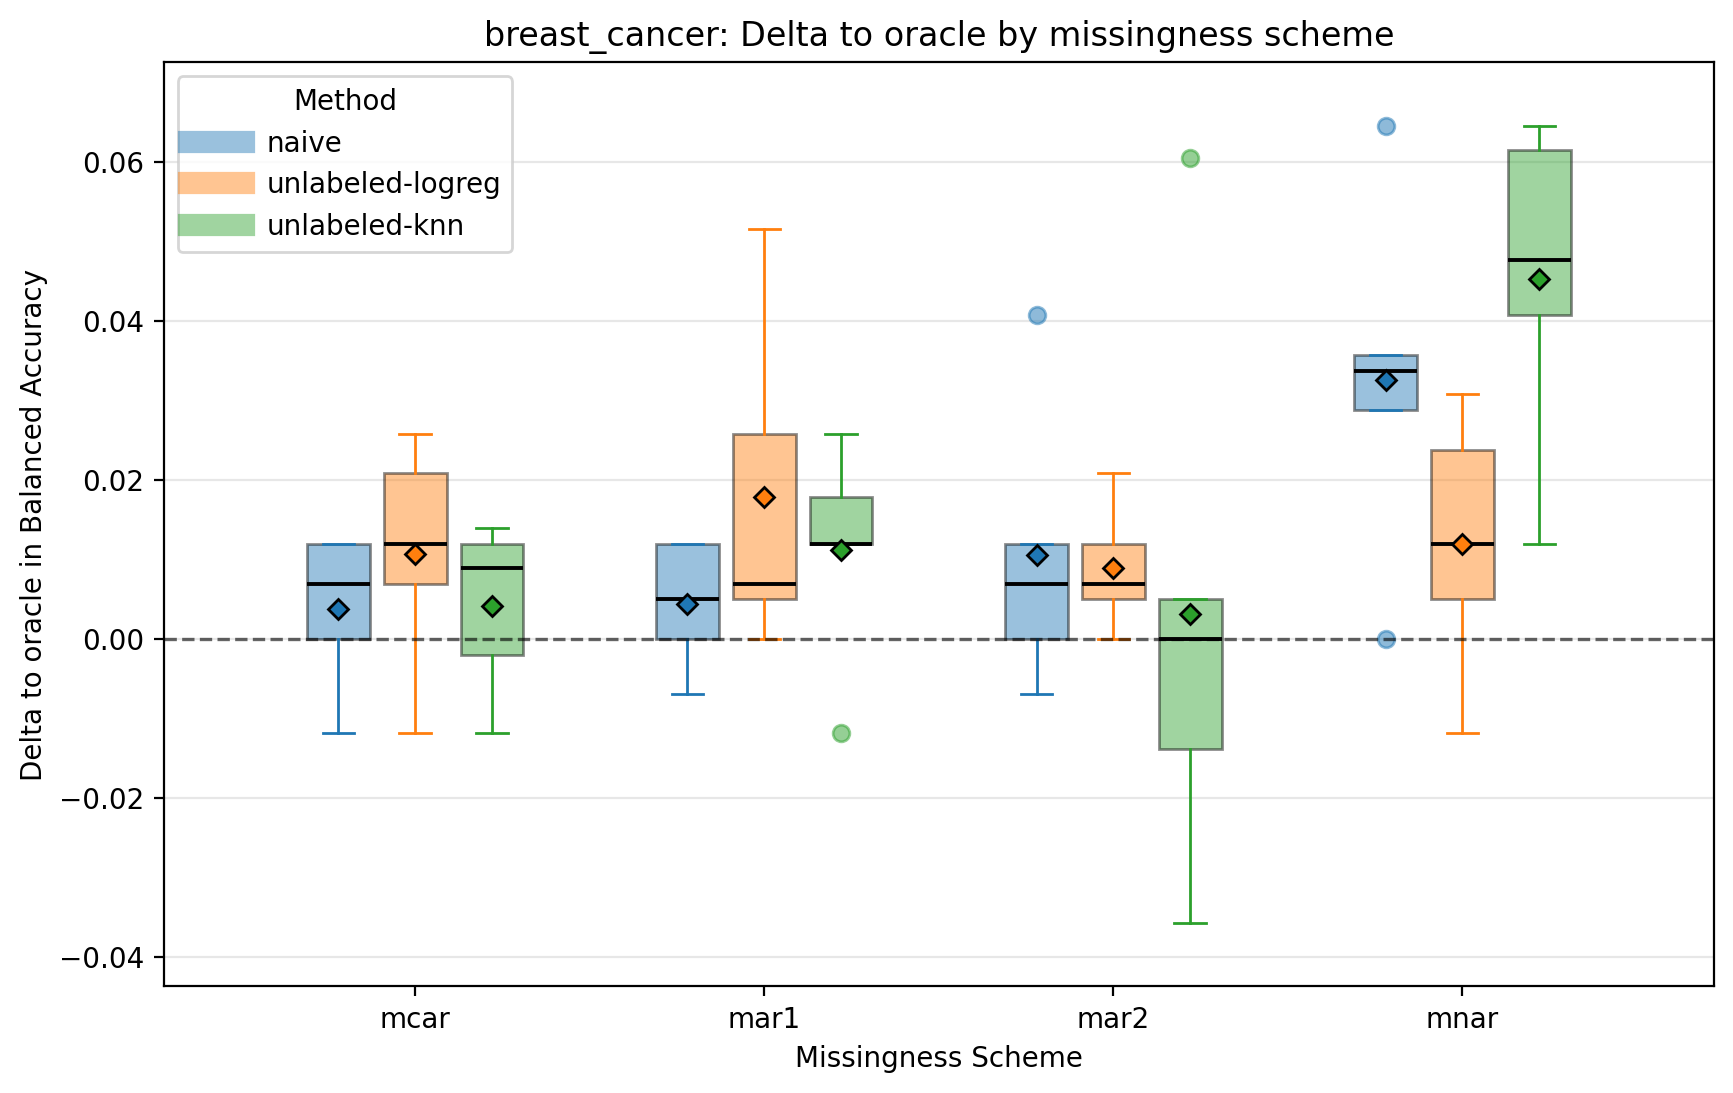
\includegraphics[width=0.75\textwidth]{../outputs/plots/breast_cancer/balanced_accuracy/delta_to_oracle_scheme.png}
    \caption{Balanced-accuracy gap to Oracle on the \texttt{breast\_cancer} dataset across all schemes at missing rate $0.3$.}
    \label{fig:scheme-breast-cancer}
\end{figure}

\paragraph{Breast cancer.}
The \texttt{breast\_cancer} dataset is the most stable setting in the study. All methods achieve high scores, and the Oracle model remains the strongest reference across all missingness mechanisms. As shown in Figure~\ref{fig:scheme-breast-cancer}, the Naive method is already very competitive under \texttt{MAR1} and also under \texttt{MCAR} at missing rate $0.3$, which suggests that this dataset is relatively robust to moderate label loss. Under \texttt{MAR2}, the unlabeled variant with kNN completion slightly improves over Naive and comes closest to Oracle among the practical methods. Under \texttt{MNAR}, however, the logistic-completion variant becomes clearly preferable, indicating that when missingness depends on the label itself, model-based label completion is more effective than either direct fitting on observed labels or local kNN completion. Overall, the main conclusion for this dataset is that missing labels do not severely damage performance, but unlabeled logistic completion becomes useful in the hardest setting.

\begin{figure}[H]
    \centering
    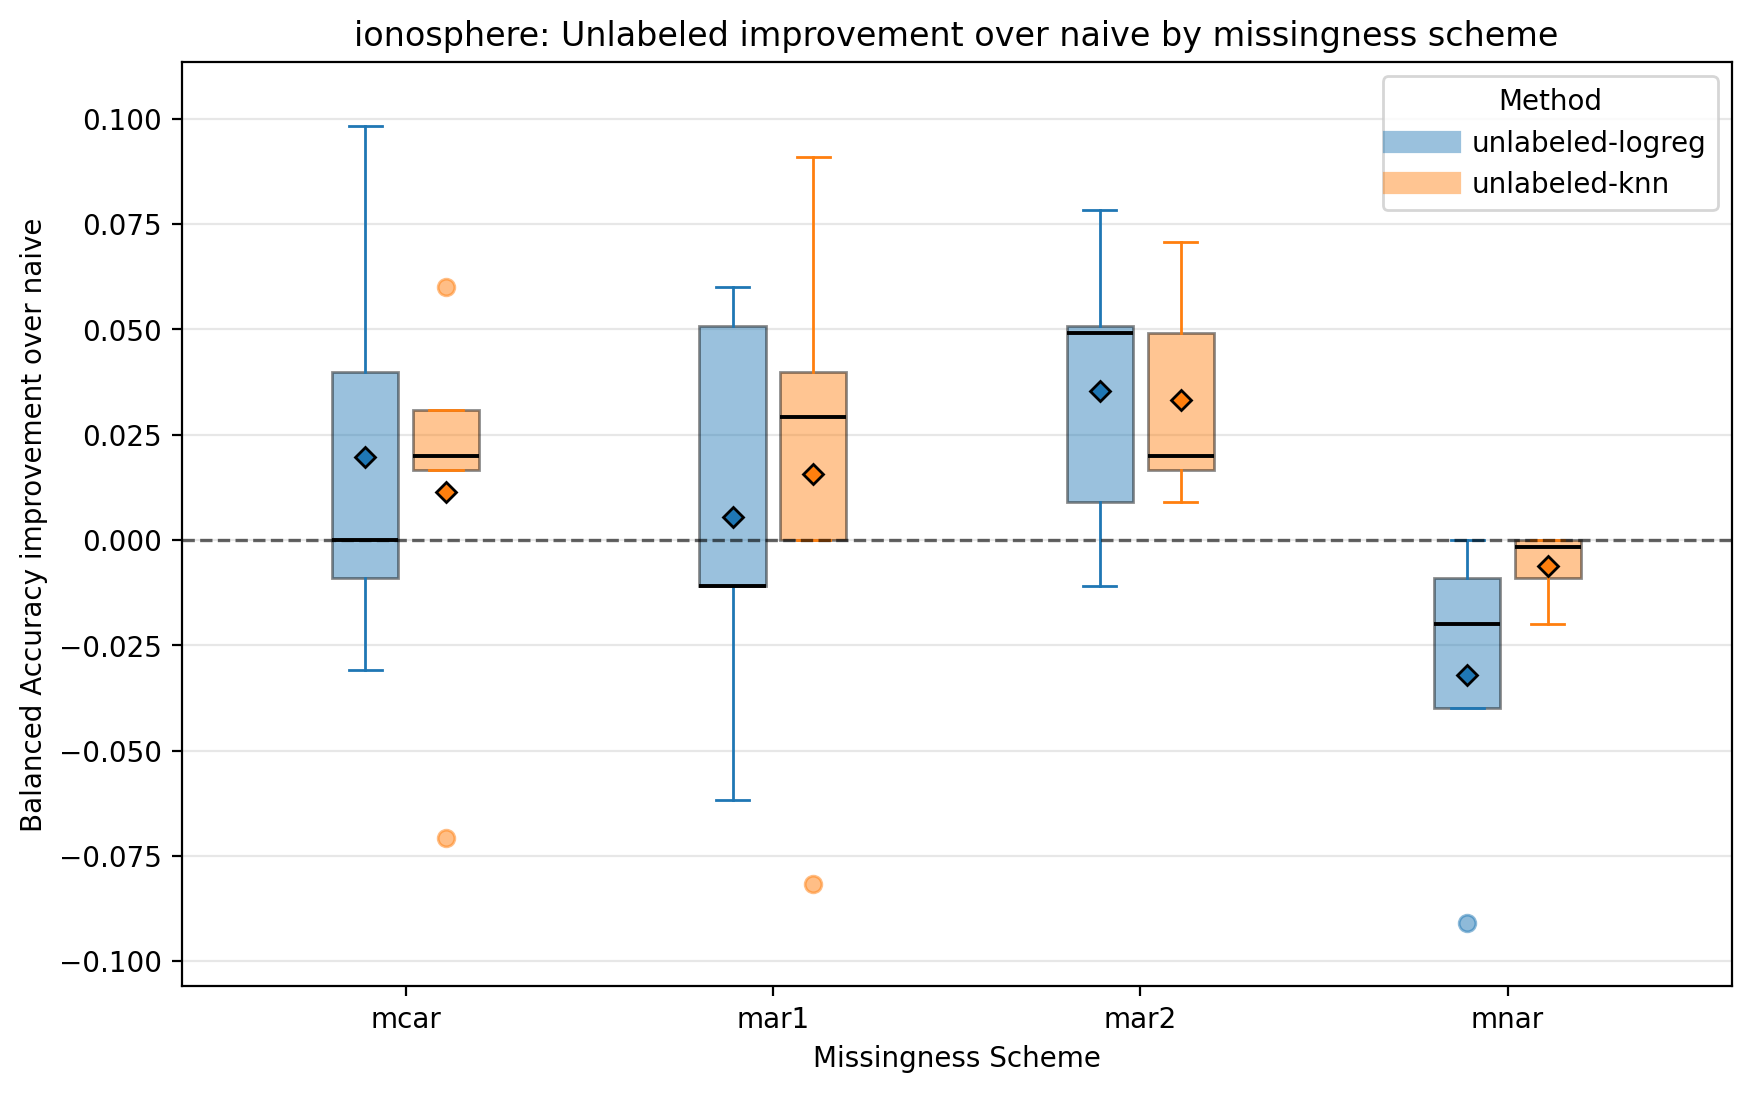
\includegraphics[width=0.75\textwidth]{../outputs/plots/ionosphere/balanced_accuracy/improvement_over_naive_scheme.png}
    \caption{Balanced-accuracy gain over Naive on the \texttt{ionosphere} dataset across all schemes.}
    \label{fig:scheme-ionosphere}
\end{figure}

\begin{figure}[H]
    \centering
    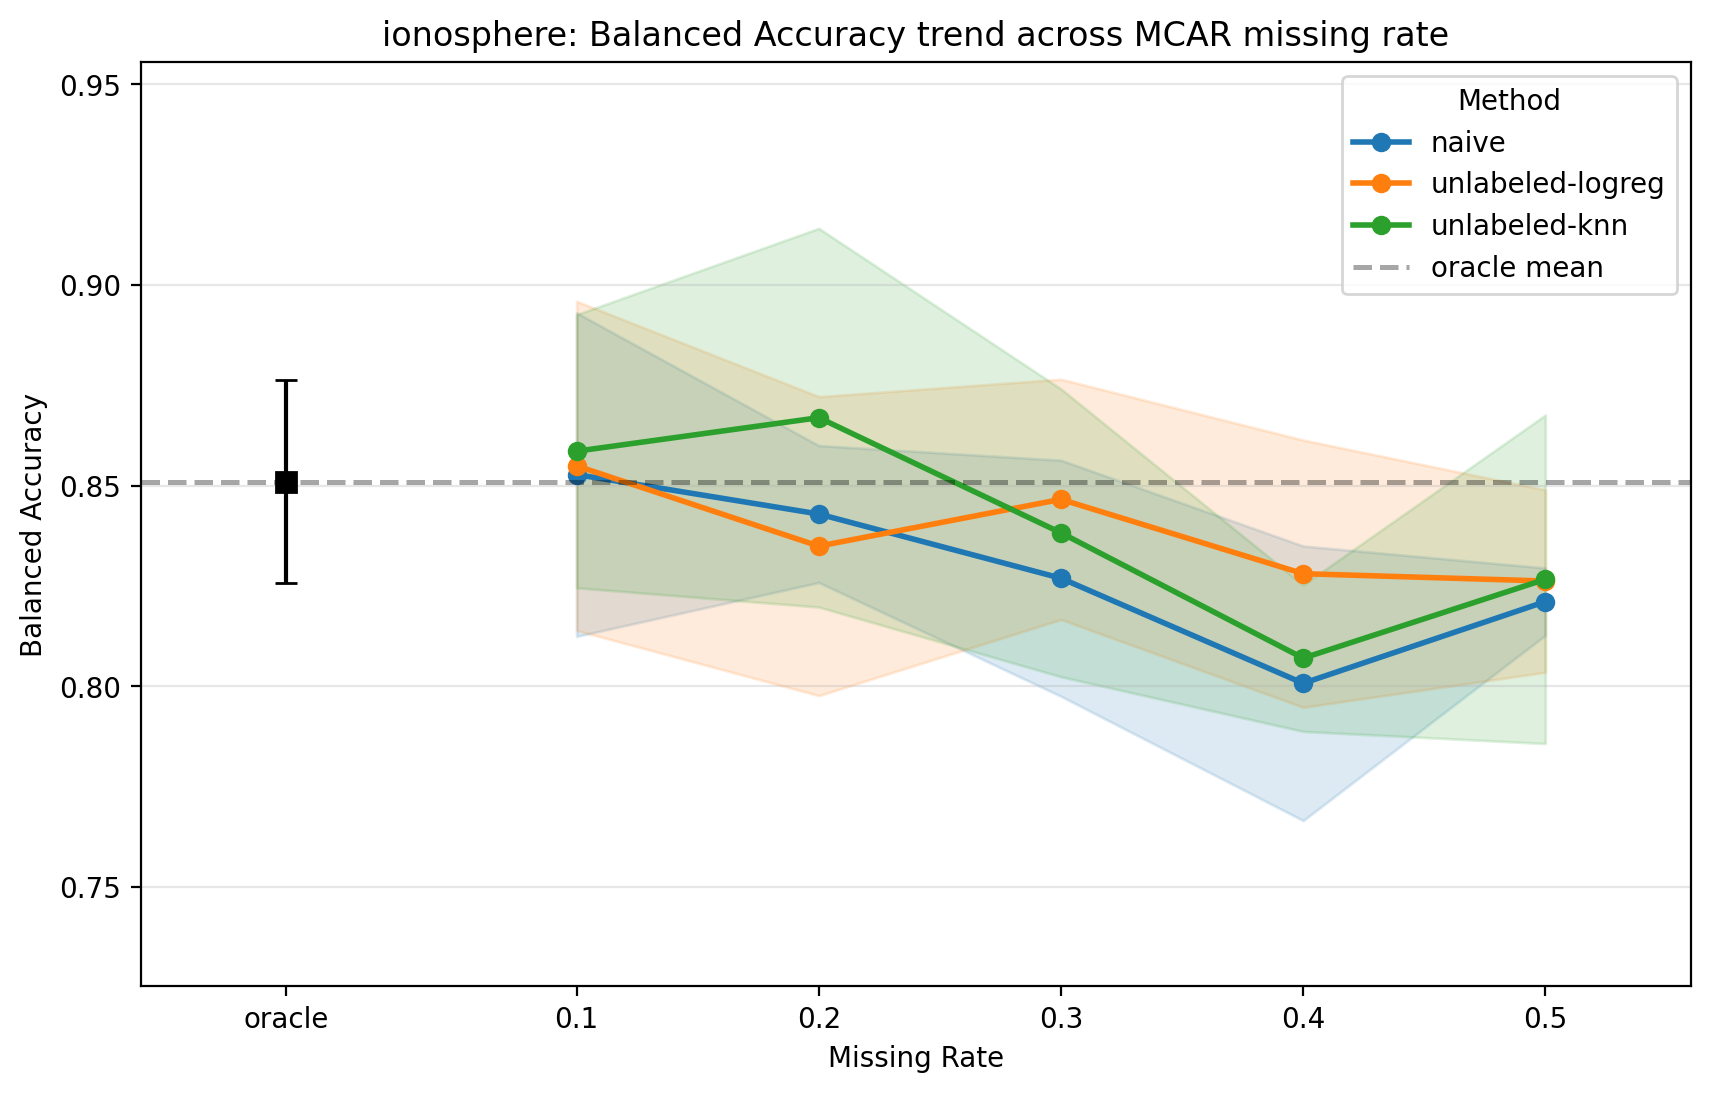
\includegraphics[width=0.75\textwidth]{../outputs/plots/ionosphere/balanced_accuracy/mcar_trend.png}
    \caption{Balanced accuracy as a function of missing rate under \texttt{MCAR} for the \texttt{ionosphere} dataset. This figure illustrates the sensitivity of the methods to increasing proportions of missing training labels.}
    \label{fig:mcar-ionosphere}
\end{figure}

\paragraph{Ionosphere.}
The \texttt{ionosphere} dataset is noticeably more sensitive to the missingness mechanism. There is no single non-Oracle method that dominates in all settings. For \texttt{MAR1}, the unlabeled method with kNN completion gives the best non-Oracle result, whereas for \texttt{MAR2}, the logistic-completion variant has the best mean balanced accuracy, although its advantage over kNN is very small. In contrast, under \texttt{MNAR}, the Naive model slightly outperforms both unlabeled variants in balanced accuracy. As shown in Figure~\ref{fig:scheme-ionosphere}, the ranking of the practical methods changes across missingness mechanisms, which suggests that the usefulness of label completion on this dataset depends strongly on how well the completion strategy matches the structure of the data. Figure~\ref{fig:mcar-ionosphere} further shows that under \texttt{MCAR} the overall performance of the non-Oracle methods declines as the missing rate increases, although the trend is not perfectly monotone. The drop is particularly visible for the Naive and kNN-based approaches, while logistic completion is somewhat more stable at higher missingness rates. Therefore, for \texttt{ionosphere}, the main message is not that one method is always best, but rather that the ranking itself depends strongly on the missingness scenario.

\begin{figure}[H]
    \centering
    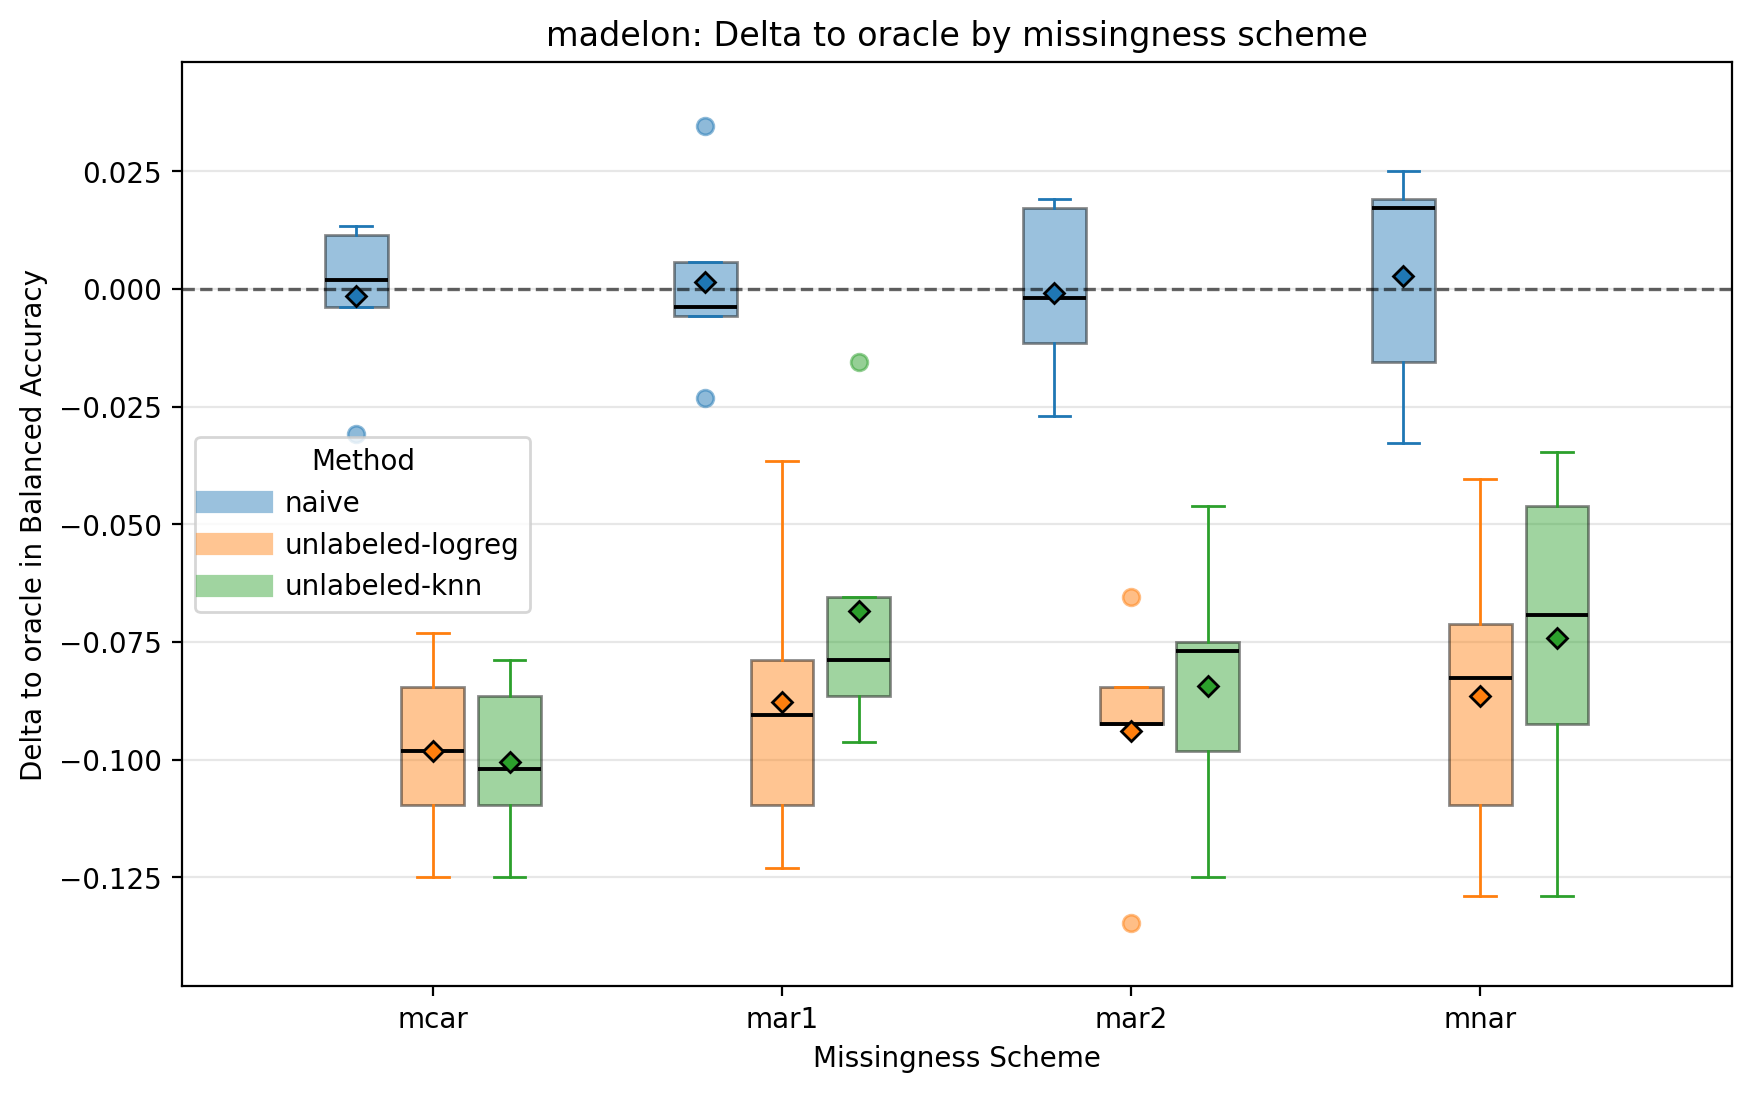
\includegraphics[width=0.75\textwidth]{../outputs/plots/madelon/balanced_accuracy/delta_to_oracle_scheme.png}
    \caption{Balanced-accuracy gap to Oracle on the \texttt{madelon} dataset across all schemes at missing rate $0.3$.}
    \label{fig:scheme-madelon}
\end{figure}

\begin{figure}[H]
    \centering
    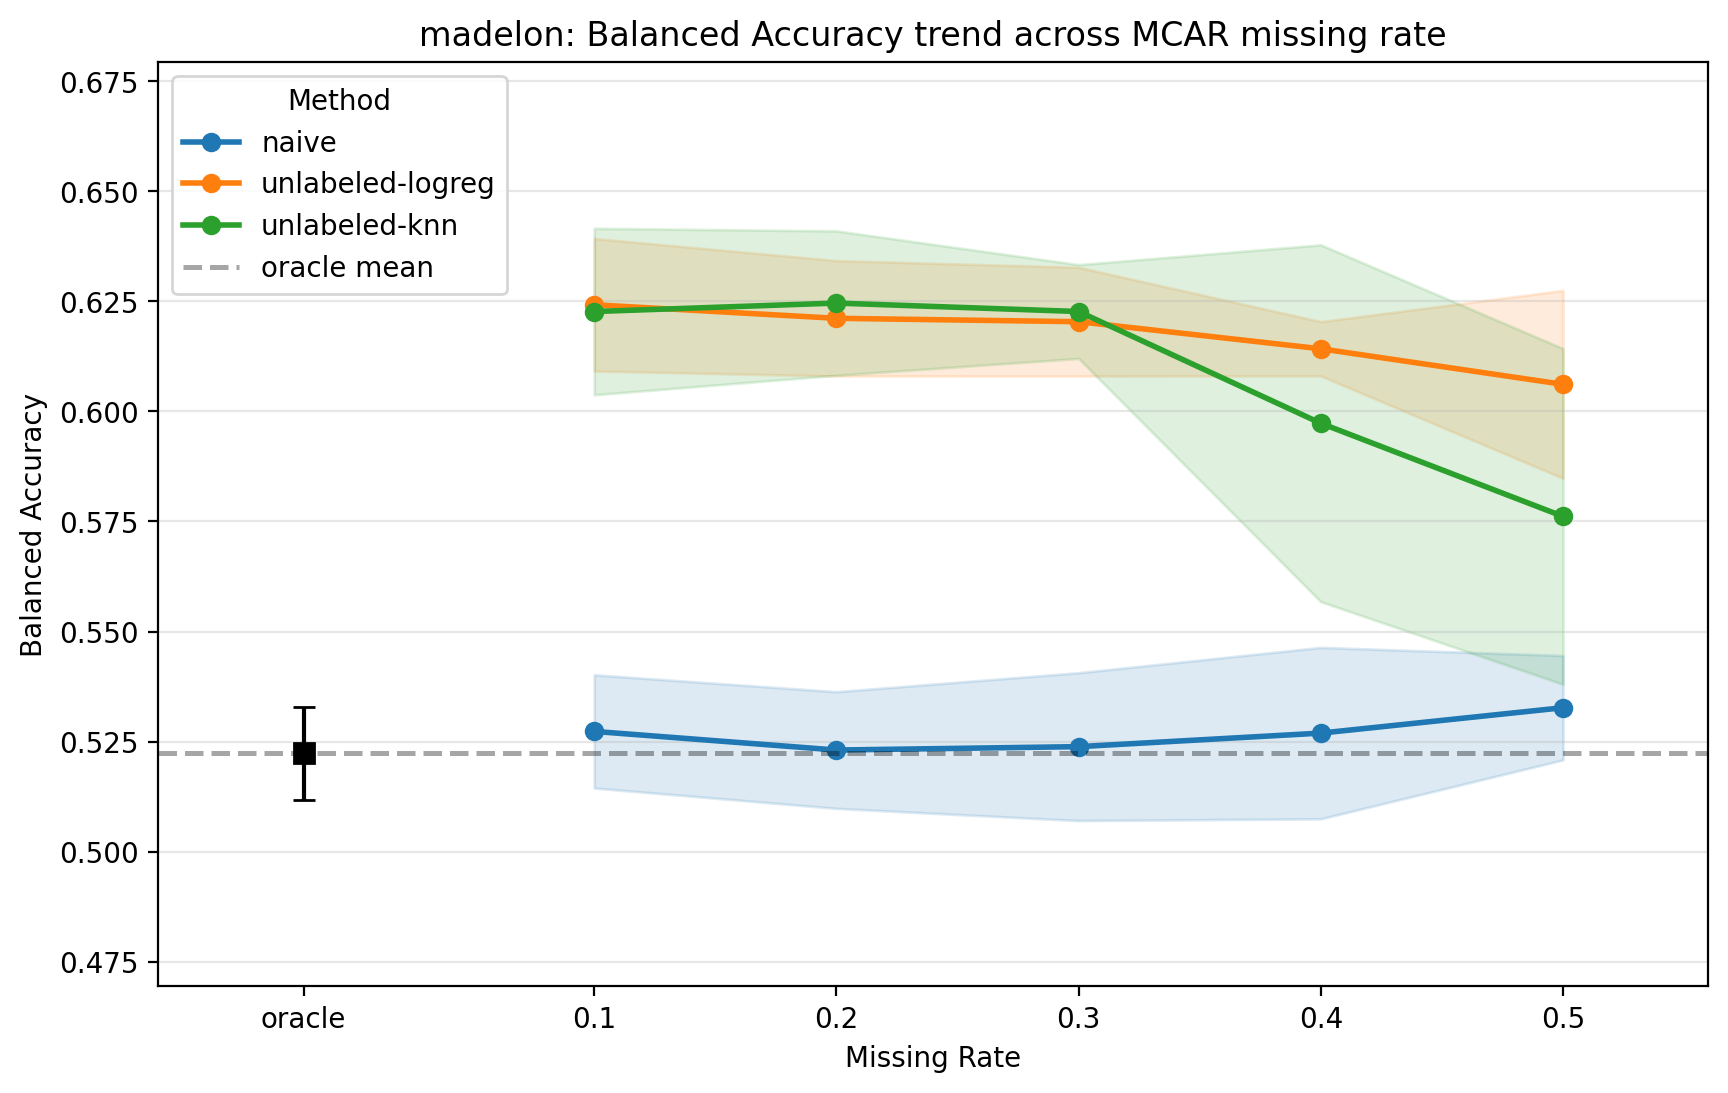
\includegraphics[width=0.75\textwidth]{../outputs/plots/madelon/balanced_accuracy/mcar_trend.png}
    \caption{Balanced accuracy under \texttt{MCAR} on the \texttt{madelon} dataset as the missing rate increases from $0.1$ to $0.5$. The unlabeled methods remain strongest, while logistic completion degrades more gradually than kNN at higher missing rates.}
    \label{fig:mcar-madelon}
\end{figure}

\paragraph{Madelon.}
The \texttt{madelon} dataset exhibits the most distinctive behavior in the entire study. Both baseline approaches, including the Oracle model, remain close to random performance, with balanced accuracy around $0.52$. In contrast, both unlabeled variants achieve substantially stronger results, and the logistic-completion method is the best approach under \texttt{MAR1}, \texttt{MAR2}, and \texttt{MNAR}. This effect is visible in Figure~\ref{fig:scheme-madelon}, where the unlabeled methods outperform the Oracle reference by a large margin. This is qualitatively different from the behavior observed on the other datasets. Under \texttt{MCAR}, the same pattern remains visible in Figure~\ref{fig:mcar-madelon}: the unlabeled methods clearly dominate for all missing rates, although their performance decreases as the fraction of missing labels grows. At low and moderate missingness, logistic and kNN completion perform similarly, but at higher missingness rates the logistic variant is more robust and degrades more smoothly. This dataset provides the strongest evidence that label completion can be beneficial when the baseline classifier struggles to learn from the raw observed labels alone.

\begin{figure}[H]
    \centering
    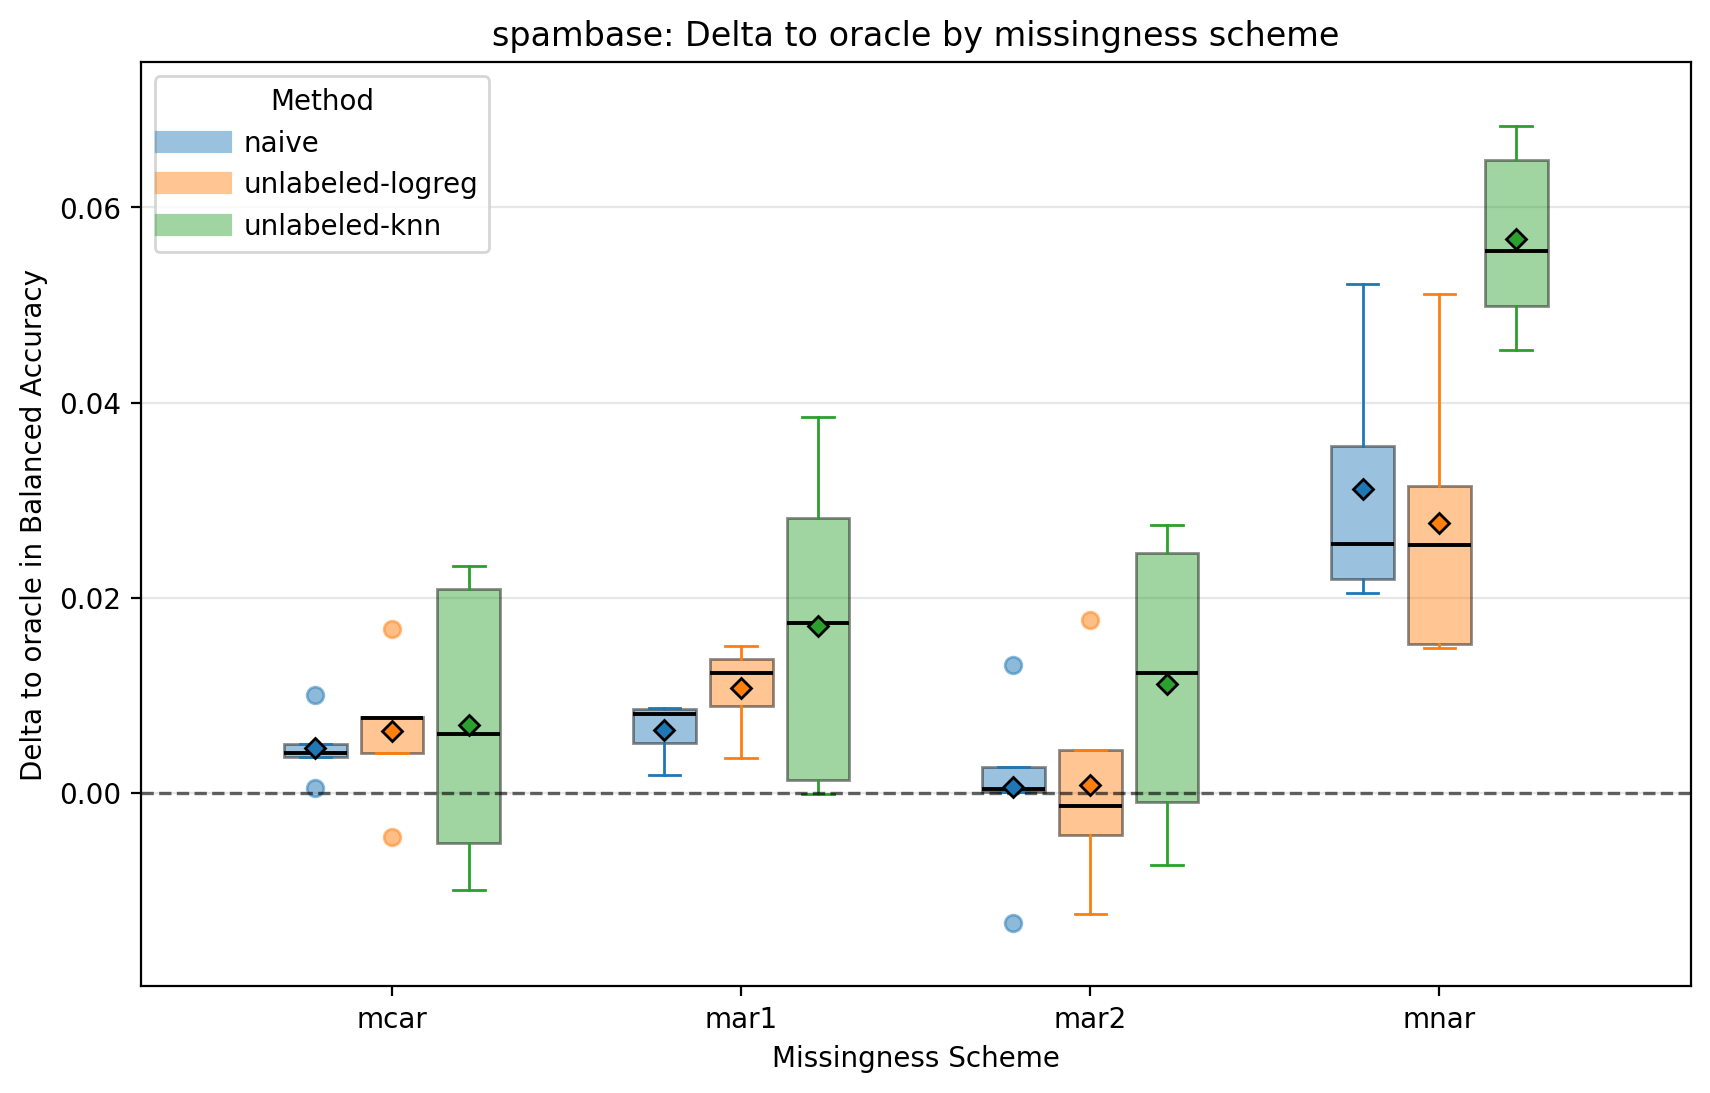
\includegraphics[width=0.75\textwidth]{../outputs/plots/spambase/balanced_accuracy/delta_to_oracle_scheme.png}
    \caption{Balanced-accuracy gap to Oracle on the \texttt{spambase} dataset across all schemes at missing rate $0.3$.}
    \label{fig:scheme-spambase}
\end{figure}

\paragraph{Spambase.}
The \texttt{spambase} dataset is similar to \texttt{breast\_cancer} in the sense that the task is comparatively easy and the Naive baseline is already very strong. Figure~\ref{fig:scheme-spambase} shows that Oracle is best overall, but the gap between Oracle and Naive is small under \texttt{MAR1}, \texttt{MAR2}, and \texttt{MCAR}. In fact, among the practical methods, Naive is the strongest non-Oracle method in these easier settings. The unlabeled approaches do not improve performance there, which suggests that when the observed labels remain sufficiently informative, direct fitting on the observed subset is already adequate. The situation changes under \texttt{MNAR}, where logistic completion becomes the best non-Oracle approach and clearly outperforms kNN completion. This again supports the broader pattern that model-based completion is most helpful when missingness depends on the true label.

\paragraph{Comparison across missingness mechanisms.}
Across datasets, \texttt{MNAR} is often among the most difficult settings, but its effect is still dataset-dependent. This is particularly visible on \texttt{breast\_cancer} and \texttt{spambase}, where the Naive and kNN-based approaches lose more performance under \texttt{MNAR} than under \texttt{MAR1} or \texttt{MAR2}, while logistic completion remains relatively more competitive. On \texttt{ionosphere}, however, \texttt{MNAR} is not uniformly the hardest setting, since the Naive model performs better there than under \texttt{MAR1} or \texttt{MAR2}. The \texttt{MAR1} and \texttt{MAR2} settings are often less harmful, although the exact ranking of methods still depends on the dataset. The results therefore indicate that the missingness mechanism is at least as important as the missingness rate itself.

\paragraph{Comparison across missing rates under MCAR.}
The \texttt{MCAR} sweep shows that robustness to increasing label loss is strongly dataset-dependent. On \texttt{breast\_cancer} and \texttt{spambase}, performance is relatively stable even when half of the training labels are missing. On \texttt{ionosphere}, the overall decline with increasing missing rate is much clearer, especially for Naive and kNN completion, although the trajectories are not strictly monotone. On \texttt{madelon}, the unlabeled methods remain best across the full range of missing rates, but both methods still decline as the amount of observed label information becomes smaller. These results confirm that there is no universal response to increasing missingness: some datasets are robust, some degrade gradually, and some show strong differences in robustness between label-completion strategies.

\paragraph{Summary of findings.}
Taken together, the results do not support a single universally best practical method. Instead, three recurring patterns emerge. First, Naive is already very strong on easier datasets such as \texttt{breast\_cancer} and \texttt{spambase}. Second, logistic label completion is most useful in harder settings and is often particularly competitive under \texttt{MNAR}. Third, the unlabeled methods are particularly effective on \texttt{madelon}, where they substantially outperform both baseline approaches.

\section{Conclusions}

The experiments show that the impact of missing labels is highly dataset-dependent, so the methods should not be compared only through a single global average. On \texttt{breast\_cancer} and \texttt{spambase}, the Naive baseline remains very competitive in many settings, especially under \texttt{MCAR}, \texttt{MAR1}, and \texttt{MAR2}. On \texttt{madelon}, however, the unlabeled methods clearly outperform both Oracle and Naive, with logistic completion emerging as the strongest approach across all missingness mechanisms considered at missing rate $0.3$. On \texttt{ionosphere}, no single non-Oracle method dominates all settings, which confirms that the usefulness of label completion depends strongly on the interaction between the missingness mechanism and the dataset structure.

A second important conclusion is that the missingness mechanism matters at least as much as the missingness rate. In particular, \texttt{MNAR} is often the hardest setting and also one of the cases in which logistic label completion becomes most beneficial. This pattern is visible on \texttt{breast\_cancer}, \texttt{spambase}, and partly on \texttt{madelon}, although \texttt{ionosphere} shows that this is not universal. Under simpler mechanisms such as \texttt{MCAR}, the benefit of unlabeled completion is smaller and sometimes disappears entirely.

The \texttt{MCAR} analysis further shows that robustness to increasing missing-label rates depends strongly on the dataset. The \texttt{breast\_cancer} and \texttt{spambase} datasets remain relatively stable even for missing rate $0.5$, whereas \texttt{ionosphere} shows a clearer overall decline as the amount of missing label information increases, despite some fluctuations across rates. On \texttt{madelon}, the unlabeled methods remain best throughout the MCAR sweep, but their performance still decreases at higher missingness rates. Among the two completion variants, logistic completion is generally more robust than kNN when the missing-label rate becomes large.

The present study also has several limitations. First, the evaluation includes only four datasets, so the conclusions should not be treated as universally valid. Second, only a small set of label-completion strategies was considered. Third, the downstream classifier family was fixed, which means that some conclusions may partly reflect the interaction between the completion method and the chosen classifier rather than the intrinsic quality of the completed labels. Finally, although five random seeds provide a reasonable basis for comparison, some settings still exhibit visible variability.

Several directions for future work are natural. The study could be extended to additional datasets with different levels of dimensionality, class imbalance, and feature redundancy. It would also be valuable to investigate more advanced label-completion strategies, including semi-supervised methods and probabilistic imputation techniques. Another promising direction would be to compare different downstream classifiers after label completion, in order to separate the effect of completion quality from the effect of the final classifier. Finally, the unusual behavior of \texttt{madelon}, where the unlabeled methods strongly outperform the Oracle baseline, deserves deeper investigation and may provide useful insight into when label completion acts as an effective form of regularization.
\clearpage
\printbibliography
\clearpage
\appendix
\section{Tables}

The table contains aggregated results from the experiments. It reports summary statistics computed across repeated runs for each dataset, missingness setting, and method.
\begin{landscape}
\footnotesize
\begin{center}
\textbf{Full summary table from \texttt{final\_summary.csv}}
\end{center}

\vspace{0.5cm}
\setlength{\LTleft}{0pt}
\setlength{\LTright}{0pt}
\csvreader[
    respect underscore,
    before reading={\setlength{\tabcolsep}{4pt}},
    after reading={\setlength{\tabcolsep}{6pt}},
    longtable={llll*{9}{r}},
    table head={
        \toprule
        dataset & scheme & method & label completion & missing rate & acc mean & acc std & bal acc mean & bal acc std & F1 mean & F1 std & ROC AUC mean & ROC AUC std\\
        \midrule
        \endfirsthead
        \toprule
        dataset & scheme & method & label completion & missing rate & acc mean & acc std & bal acc mean & bal acc std & F1 mean & F1 std & ROC AUC mean & ROC AUC std\\
        \midrule
        \endhead
        \midrule
        \multicolumn{13}{r}{Continued on next page}\\
        \endfoot
        \bottomrule
        \endlastfoot
    }
]{../outputs/tables/final_summary.csv}{}{
    \csvcoli & \csvcolii & \csvcoliii & \csvcoliv &
    \tablevalue{\csvcolv} &
    \tablevalue{\csvcolvi} &
    \tablevalue{\csvcolvii} &
    \tablevalue{\csvcolviii} &
    \tablevalue{\csvcolix} &
    \tablevalue{\csvcolx} &
    \tablevalue{\csvcolxi} &
    \tablevalue{\csvcolxii} &
    \tablevalue{\csvcolxiii}
}
\end{landscape}

\clearpage
\section{Figures}

This appendix contains balanced-accuracy plots that were not included in the main text.

\newcommand{\balappendixplot}[3]{
\begin{figure}[H]
    \centering
    \includegraphics[width=0.82\textwidth]{../outputs/plots/#1/balanced_accuracy/#2.png}
    \caption{#3}
\end{figure}
}

\subsection{Breast cancer}

\balappendixplot{breast_cancer}{delta_to_oracle_missing_rate}
{Balanced-accuracy gap to Oracle on the \texttt{breast\_cancer} dataset under \texttt{MCAR} as missing rate varies.}

\balappendixplot{breast_cancer}{delta_to_oracle_missing_rate_boxplot}
{Balanced-accuracy gap to Oracle on the \texttt{breast\_cancer} dataset across MCAR missing rates.}

\balappendixplot{breast_cancer}{improvement_over_naive_missing_rate}
{Balanced-accuracy gain over Naive on the \texttt{breast\_cancer} dataset under \texttt{MCAR} as missing rate varies.}

\balappendixplot{breast_cancer}{improvement_over_naive_missing_rate_boxplot}
{Balanced-accuracy gain over Naive on the \texttt{breast\_cancer} dataset across MCAR missing rates.}

\balappendixplot{breast_cancer}{improvement_over_naive_scheme}
{Balanced-accuracy gain over Naive on the \texttt{breast\_cancer} dataset across all schemes.}

\balappendixplot{breast_cancer}{mcar_trend}
{Balanced accuracy on the \texttt{breast\_cancer} dataset under \texttt{MCAR} for different missing rates.}

\balappendixplot{breast_cancer}{methods_boxplot}
{Balanced accuracy on the \texttt{breast\_cancer} dataset: comparison of methods across experimental settings.}

\balappendixplot{breast_cancer}{missing_rate_boxplot}
{Balanced accuracy on the \texttt{breast\_cancer} dataset: distribution across missing rates.}

\clearpage
\subsection{Ionosphere}

\balappendixplot{ionosphere}{delta_to_oracle_missing_rate}
{Balanced-accuracy gap to Oracle on the \texttt{ionosphere} dataset under \texttt{MCAR} as missing rate varies.}

\balappendixplot{ionosphere}{delta_to_oracle_missing_rate_boxplot}
{Balanced-accuracy gap to Oracle on the \texttt{ionosphere} dataset across MCAR missing rates.}

\balappendixplot{ionosphere}{delta_to_oracle_scheme}
{Balanced-accuracy gap to Oracle on the \texttt{ionosphere} dataset across all schemes.}

\balappendixplot{ionosphere}{improvement_over_naive_missing_rate}
{Balanced-accuracy gain over Naive on the \texttt{ionosphere} dataset under \texttt{MCAR} as missing rate varies.}

\balappendixplot{ionosphere}{improvement_over_naive_missing_rate_boxplot}
{Balanced-accuracy gain over Naive on the \texttt{ionosphere} dataset across MCAR missing rates.}

\balappendixplot{ionosphere}{improvement_over_naive_scheme}
{Balanced-accuracy gain over Naive on the \texttt{ionosphere} dataset across all schemes.}

\balappendixplot{ionosphere}{methods_boxplot}
{Balanced accuracy on the \texttt{ionosphere} dataset: comparison of methods across experimental settings.}

\balappendixplot{ionosphere}{missing_rate_boxplot}
{Balanced accuracy on the \texttt{ionosphere} dataset: distribution across missing rates.}

\clearpage
\subsection{Madelon}

\balappendixplot{madelon}{delta_to_oracle_missing_rate}
{Balanced-accuracy gap to Oracle on the \texttt{madelon} dataset under \texttt{MCAR} as missing rate varies.}

\balappendixplot{madelon}{delta_to_oracle_missing_rate_boxplot}
{Balanced-accuracy gap to Oracle on the \texttt{madelon} dataset across MCAR missing rates.}

\balappendixplot{madelon}{improvement_over_naive_missing_rate}
{Balanced-accuracy gain over Naive on the \texttt{madelon} dataset under \texttt{MCAR} as missing rate varies.}

\balappendixplot{madelon}{improvement_over_naive_missing_rate_boxplot}
{Balanced-accuracy gain over Naive on the \texttt{madelon} dataset across MCAR missing rates.}

\balappendixplot{madelon}{improvement_over_naive_scheme}
{Balanced-accuracy gain over Naive on the \texttt{madelon} dataset across all schemes.}

\balappendixplot{madelon}{methods_boxplot}
{Balanced accuracy on the \texttt{madelon} dataset: comparison of methods across experimental settings.}

\balappendixplot{madelon}{missing_rate_boxplot}
{Balanced accuracy on the \texttt{madelon} dataset: distribution across missing rates.}

\clearpage
\subsection{Spambase}

\balappendixplot{spambase}{delta_to_oracle_missing_rate}
{Balanced-accuracy gap to Oracle on the \texttt{spambase} dataset under \texttt{MCAR} as missing rate varies.}

\balappendixplot{spambase}{delta_to_oracle_missing_rate_boxplot}
{Balanced-accuracy gap to Oracle on the \texttt{spambase} dataset across MCAR missing rates.}

\balappendixplot{spambase}{improvement_over_naive_missing_rate}
{Balanced-accuracy gain over Naive on the \texttt{spambase} dataset under \texttt{MCAR} as missing rate varies.}

\balappendixplot{spambase}{improvement_over_naive_missing_rate_boxplot}
{Balanced-accuracy gain over Naive on the \texttt{spambase} dataset across MCAR missing rates.}

\balappendixplot{spambase}{improvement_over_naive_scheme}
{Balanced-accuracy gain over Naive on the \texttt{spambase} dataset across all schemes.}

\balappendixplot{spambase}{mcar_trend}
{Balanced accuracy on the \texttt{spambase} dataset under \texttt{MCAR} for different missing rates.}

\balappendixplot{spambase}{methods_boxplot}
{Balanced accuracy on the \texttt{spambase} dataset: comparison of methods across experimental settings.}

\balappendixplot{spambase}{missing_rate_boxplot}
{Balanced accuracy on the \texttt{spambase} dataset: distribution across missing rates.}

\end{document}
